\documentclass[12pt, a4paper]{book}

\usepackage[T1]{fontenc}
\usepackage[utf8]{inputenc}
\usepackage[charter, cal=cmcal]{mathdesign}
\usepackage[scaled=0.92]{helvet}
\usepackage{geometry}
\geometry{a4paper, top=30mm, bottom=30mm, inner=32mm, outer=25mm, marginparwidth=18mm}

\usepackage{amsmath, amsthm}
\usepackage[version=4]{mhchem}
\usepackage{graphicx}
\usepackage{xcolor}
\usepackage{tikz}
\usetikzlibrary{arrows.meta, shapes.geometric, positioning, calc, backgrounds}
\usepackage{pgfplots}
\pgfplotsset{compat=1.18}
\usepackage{tcolorbox}
\tcbuselibrary{skins, breakable, theorems}
\usepackage{titlesec}
\usepackage{fancyhdr}
\usepackage{enumitem}
\usepackage{booktabs}
\usepackage{array}
\usepackage{parskip}
\usepackage{siunitx}
\usepackage[colorlinks=true, linkcolor=BrickRed,
            urlcolor=NavyBlue, citecolor=ForestGreen]{hyperref}

% ── Colours (Charcoal / Royal Blue) ──────────────────────────────────────────
\definecolor{JourneyColor}{HTML}{0F172A}
\definecolor{ModuleColor}{HTML}{2563EB}
\definecolor{PuzzleColor}{HTML}{D97706}
\definecolor{DiscoveryColor}{HTML}{3B82F6}
\definecolor{WarningColor}{HTML}{991B1B}
\definecolor{ProblemColor}{HTML}{6B21A8}
\definecolor{ReflectColor}{HTML}{0D9488}
\definecolor{HistoryColor}{HTML}{78350F}

% ── Boxes ─────────────────────────────────────────────────────────────────────
\newtcolorbox{puzzlebox}[1][]{enhanced,breakable,
  colback=PuzzleColor!6,colframe=PuzzleColor,fonttitle=\bfseries\sffamily,
  title={The Puzzle},attach boxed title to top left={yshift=-2mm,xshift=6mm},
  boxed title style={colback=PuzzleColor},borderline west={3pt}{0pt}{PuzzleColor},#1}

\newtcolorbox{discoverybox}[1][]{enhanced,breakable,
  colback=DiscoveryColor!8,colframe=DiscoveryColor,fonttitle=\bfseries\sffamily,
  title={Discovery},attach boxed title to top left={yshift=-2mm,xshift=6mm},
  boxed title style={colback=DiscoveryColor},borderline west={3pt}{0pt}{DiscoveryColor},#1}

\newtcolorbox{problembox}[1][]{enhanced,breakable,
  colback=ProblemColor!5,colframe=ProblemColor,fonttitle=\bfseries\sffamily,
  title={Problems},attach boxed title to top left={yshift=-2mm,xshift=6mm},
  boxed title style={colback=ProblemColor},borderline west={3pt}{0pt}{ProblemColor},#1}

\newtcolorbox{deepbox}[1][]{enhanced,breakable,
  colback=JourneyColor!5,colframe=JourneyColor,fonttitle=\bfseries\sffamily,
  title={Deep Problems},attach boxed title to top left={yshift=-2mm,xshift=6mm},
  boxed title style={colback=JourneyColor},borderline west={4pt}{0pt}{JourneyColor},#1}

\newtcolorbox{historybox}[1][]{enhanced,breakable,
  colback=HistoryColor!7,colframe=HistoryColor!60,fonttitle=\bfseries\sffamily\small,
  title={Historical Note},attach boxed title to top left={yshift=-2mm,xshift=6mm},
  boxed title style={colback=HistoryColor!80},#1}

\newtcolorbox{reflectionbox}[1][]{enhanced,breakable,
  colback=ReflectColor!6,colframe=ReflectColor,fonttitle=\bfseries\sffamily,
  title={Reflection},attach boxed title to top left={yshift=-2mm,xshift=6mm},
  boxed title style={colback=ReflectColor},borderline west={3pt}{0pt}{ReflectColor},#1}

\newtcolorbox{namedconcept}[2][]{enhanced,
  colback=ModuleColor!6,colframe=ModuleColor,fonttitle=\bfseries\sffamily\large,
  title={#2},attach boxed title to top left={yshift=-2mm,xshift=6mm},
  boxed title style={colback=ModuleColor},#1}

% ── Section formatting ────────────────────────────────────────────────────────
\titleformat{\chapter}[display]
  {\normalfont\sffamily\huge\bfseries\color{JourneyColor}}
  {\textcolor{JourneyColor!60}{\chaptertitlename\ \thechapter}}{10pt}{\Huge}
  [\vspace{2pt}\textcolor{JourneyColor}{\titlerule[1.5pt]}]
\titleformat{\section}
  {\normalfont\sffamily\Large\bfseries\color{ModuleColor}}
  {\thesection}{1em}{}[\textcolor{ModuleColor!40}{\titlerule[0.6pt]}]
\titleformat{\subsection}
  {\normalfont\sffamily\large\bfseries\color{JourneyColor!80}}{\thesubsection}{1em}{}
\titleformat{\subsubsection}
  {\normalfont\sffamily\normalsize\bfseries}{\thesubsubsection}{1em}{}

\pagestyle{fancy}
\fancyhf{}
\fancyhead[LE]{\small\sffamily\textcolor{JourneyColor}{\leftmark}}
\fancyhead[RO]{\small\sffamily\textcolor{ModuleColor}{\rightmark}}
\fancyfoot[C]{\small\thepage}
\renewcommand{\headrulewidth}{0.4pt}

\newcommand{\newterm}[1]{\textit{\textcolor{DiscoveryColor}{#1}}}
\newcommand{\important}[1]{\textcolor{ModuleColor}{\textbf{#1}}}

\begin{document}

\setcounter{chapter}{3}
\chapter[Journey 4 --- Programming Paradigms and Language Semantics]
        {Journey Four\\[8pt]
         \textcolor{ModuleColor}{\large Programming Paradigms and Language Semantics}}
\setcounter{section}{3}

\section{Module 4.4 --- Compiler Design: Parsing to Code Generation}
\label{sec:mod4.4}

\subsection*{Motivation}

We completed in Module 4.3 the mathematical logic of types, proving that type constraints statically guarantee program safety.
But code and types are still abstract mathematical terms.
To run our code, we must translate these high-level descriptions into the physical switches of the processor datapath that we designed in Journey 2.
This translation is executed by a **Compiler**.

A compiler is a complex pipeline that transforms a flat sequence of characters into a structured tree, performs semantic verification, optimizes the code, and generates machine assembly.
This module explores each stage of the compiler pipeline: from lexical scanners and syntax parsers to Intermediate Representations and target code generation.
We will discover how NP-complete graph coloring algorithms manage hardware registers, and how the compilation process bridges abstract language and physical hardware.

\subsection{The Arithmetic Evaluator}

We analyze how flat strings of characters are parsed into logic structures.

\begin{puzzlebox}
\textbf{The Character Stream.}

Suppose a programmer writes the following expression in a code file:
\[
  \text{result} \;=\; 3 + 4 \times (5 - x)
\]
To a physical processor, this code is initially just a flat stream of characters: `['r', 'e', 's', 'u', 'l', 't', ' ', '=', ' ', '3', ' ', '+', ' ', '4', ' ', '*', ' ', '(', '5', ' ', '-', ' ', 'x', ')']`.
\begin{enumerate}[label=(\alph*), leftmargin=*]
  \item The first stage, **Lexical Analysis (Scanning)**, converts this stream of characters into a stream of classified **tokens** (e.g. `IDENT("result")`, `ASSIGN`, `INT(3)`, `PLUS`, `INT(4)`, `TIMES`, `LPAREN`, `INT(5)`, `MINUS`, `IDENT("x")`, `RPAREN`).
        Explain how finite automata (DFAs from Journey 3 Module 3.1) are used to recognize these tokens.
  \item The second stage, **Syntax Analysis (Parsing)**, groups these tokens into a hierarchical **Abstract Syntax Tree (AST)**.
        Draw the AST for this expression, showing how the tree structure enforces the standard precedence of parentheses, multiplication, and addition.
  \item The final stage, **Code Generation**, translates the AST into a sequence of binary machine instructions.
        Write down a sequence of pseudocode assembly instructions (using registers $R_0, R_1, R_2$) that evaluates this tree.
\end{enumerate}
\end{puzzlebox}

\subsection{The Compiler Pipeline and Parsing Strategies}

We explore the parsing and semantic analysis phases.

\begin{center}
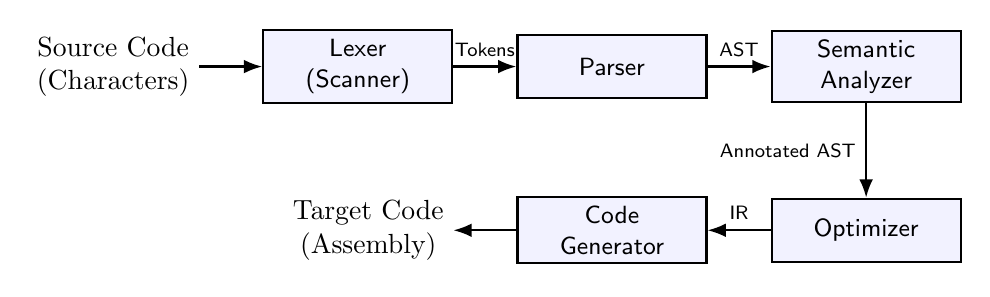
\begin{tikzpicture}[
  node distance=1.2cm and 0.8cm,
  box/.style={draw, thick, fill=blue!5, minimum width=2.4cm, minimum height=0.8cm, align=center, font=\small\sffamily},
  arrow/.style={-Latex, thick}
]
  \node (char) [align=center] {Source Code\\(Characters)};
  \node (lex) [box, right=of char] {Lexer\\(Scanner)};
  \node (parse) [box, right=of lex] {Parser};
  \node (sem) [box, right=of parse] {Semantic\\Analyzer};
  \node (opt) [box, below=1.2cm of sem] {Optimizer};
  \node (codegen) [box, left=of opt] {Code\\Generator};
  \node (asm) [align=center, left=of codegen] {Target Code\\(Assembly)};

  \draw [arrow] (char) -- (lex);
  \draw [arrow] (lex) -- node[above, font=\scriptsize\sffamily] {Tokens} (parse);
  \draw [arrow] (parse) -- node[above, font=\scriptsize\sffamily] {AST} (sem);
  \draw [arrow] (sem) -- node[left, font=\scriptsize\sffamily] {Annotated AST} (opt);
  \draw [arrow] (opt) -- node[above, font=\scriptsize\sffamily] {IR} (codegen);
  \draw [arrow] (codegen) -- (asm);
\end{tikzpicture}
\end{center}

\begin{explobox}
Parsers are governed by Context-Free Grammars (from Journey 3 Module 3.2). There are two primary parsing strategies:
1. **Top-Down Parsing (LL):** Builds the parse tree starting from the start symbol and expanding down to the leaves, using a lookup table to select the next rule based on lookahead tokens.
2. **Bottom-Up Parsing (LR):** Builds the tree from the leaves up to the start symbol, using a pushdown stack to shift tokens and reduce matching patterns.
\begin{enumerate}[label=(\alph*), leftmargin=*]
  \item Why does a top-down LL parser fail on grammars that contain **left recursion** (rules like $A \to A + B$)? (What happens to a recursive descent function when it encounters this rule?)
  \item During the **Semantic Analysis** phase, the compiler traverses the AST to check rules that cannot be captured by context-free grammars.
        Give three examples of semantic rules verified during this phase (e.g. verifying variables are declared before use).
  \item Why does type checking (using the typing rules from Module 4.3) occur during this semantic phase rather than the syntax parsing phase?
\end{enumerate}
\end{explobox}

\subsection{Code Generation and Register Allocation}

We study how compilers optimize code and map variables to finite hardware registers.

\begin{explobox}
Before generating machine code, compilers translate the AST into an **Intermediate Representation (IR)** such as Three-Address Code, where each instruction has at most one operator and three operands: $x := y \text{ op } z$.
* **Register Allocation:** A physical CPU has a very small number of registers (e.g. 16 registers). The compiler must map an infinite number of temporary variables in the IR code to these 16 registers.
* **Chaitin's Formulation:** We construct an **Interference Graph**, where each node is a variable, and an edge connects two nodes if they are "live" simultaneously (meaning both variables hold active values at the same program step). Register allocation is equivalent to the **$k$-coloring problem** of this graph, where $k$ is the number of registers.
\begin{enumerate}[label=(\alph*), leftmargin=*]
  \item Since $k$-coloring is an NP-complete problem (from Journey 3 Module 3.4), how do compilers handle cases where a graph cannot be colored using $k$ colors? (What is a register **spill**?)
  \item Consider the following three-address code steps:
        ```
          Step 1: A := 5
          Step 2: B := 10
          Step 3: C := A + B
          Step 4: D := C * 2
        ```
        Draw the interference graph for the variables $A, B, C, D$.
  \item What is the minimum number of registers required to execute this code without memory spills?
\end{enumerate}
\end{explobox}

\newpage

% ─── Section: Discovery ──────────────────────────────────────────────────────
\section{Part 3 --- Discovery}

\begin{discoverybox}
\textbf{What have we built?}

\textbf{First.} The compiler pipeline transforms source code through scanning, parsing, semantic analysis, optimization, and code generation.

\textbf{Second.} Scanning uses DFAs to group characters into tokens. Parsing uses context-free grammars (LL or LR strategies) to build Abstract Syntax Trees.

\textbf{Third.} Register allocation uses Chaitin's graph coloring heuristic to solve the NP-complete mapping of variable lifetimes to physical hardware registers.

\textbf{Fourth.} Static Single Assignment (SSA) form assigns every variable exactly once, utilizing $\phi$-nodes at control junctions to simplify code optimizations.
\end{discoverybox}

\newpage

% ─── Section: Naming Concepts ────────────────────────────────────────────────
\section{Part 4 --- What This Is Called}

\begin{namedconcept}{Compiler parameters}
* **Lexer (Scanner):** The compiler component that groups input characters into classified tokens.
* **Parser:** The compiler component that parses tokens into an Abstract Syntax Tree (AST) using a grammar.
* **Abstract Syntax Tree (AST):** A tree representation of the hierarchical syntactic structure of source code.
* **Intermediate Representation (IR):** A machine-independent code format (like three-address code) used for optimization.
* **Register Allocation:** The process of mapping program variables to a finite number of CPU registers.
* **Static Single Assignment (SSA):** An IR format where each variable is assigned exactly once.
\end{namedconcept}

\newpage

% ─── Section: Solved Exercises ───────────────────────────────────────────────
\section{Part 5 --- Solved Exercises}

\begin{problembox}
\begin{enumerate}[label=\textbf{E\arabic*.}]
  \item \textbf{Drawing an Abstract Syntax Tree.}
  
        Draw the Abstract Syntax Tree (AST) for the statement:
        \[
          \text{result} \;=\; 3 + 4 \times (5 - x).
        \]
        
        \textbf{Solution:}
        An AST represents the operators as parent nodes and the operands as child nodes.
        The operations must be nested to respect the order of precedence:
        1. Subtraction $(5 - x)$ has highest priority because of the parentheses.
        2. Multiplication $4 \times (5 - x)$ has next priority.
        3. Addition $3 + (4 \times (5 - x))$ has next priority.
        4. Assignment $\text{result} = \text{addition\_result}$ has the lowest priority.
        
        Let us draw the hierarchical tree structure:
        \begin{center}
        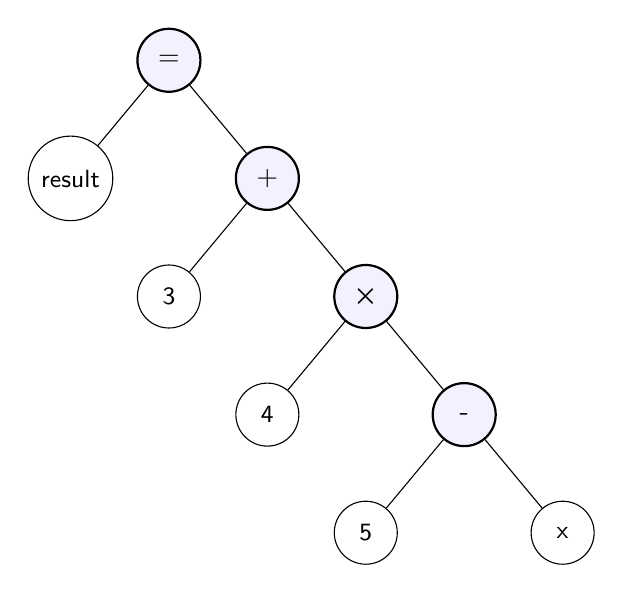
\begin{tikzpicture}[
          level distance=1.5cm,
          sibling distance=2.5cm,
          node/.style={circle, draw, thick, fill=blue!5, minimum size=0.8cm, font=\sffamily\boldmath}
        ]
          \node[node] (assign) {=}
            child { node[circle, draw, minimum size=0.8cm, font=\small\sffamily] {result} }
            child { node[node] (add) {+}
              child { node[circle, draw, minimum size=0.8cm, font=\small\sffamily] {3} }
              child { node[node] (mul) {$\times$}
                child { node[circle, draw, minimum size=0.8cm, font=\small\sffamily] {4} }
                child { node[node] (sub) {-}
                  child { node[circle, draw, minimum size=0.8cm, font=\small\sffamily] {5} }
                  child { node[circle, draw, minimum size=0.8cm, font=\small\sffamily] {x} }
                }
              }
            };
        \end{tikzpicture}
        \end{center}
        This AST correctly represents the expression structure.
        
  \item \textbf{Translating to Three-Address Code.}
  
        Translate the following high-level code snippet into equivalent Three-Address Code:
        ```
          y := x + 1;
          z := y * 2;
          if (z > 10) then
              w := z
          else
              w := 0;
        ```
        
        \textbf{Solution:}
        Three-Address Code (3AC) represents instructions with at most one operator and three operands.
        We can implement control flow (if-then-else) using conditional jumps and label markers.
        
        Let us translate the snippet step-by-step:
        ```
          t1 := x + 1
          y := t1
          t2 := y * 2
          z := t2
          if z <= 10 goto L1
          w := z
          goto L2
          L1:
          w := 0
          L2:
        ```
        Here, `t1` and `t2` are compiler-generated temporary variables, and `L1` and `L2` are code labels. This 3AC correctly preserves the logic of the original code.
\end{enumerate}
\end{problembox}

\newpage

% ─── Section: Problems ───────────────────────────────────────────────────────
\section{Part 6 --- Problems}

\begin{problembox}
\begin{enumerate}[label=\textbf{P\arabic*.}]
  \item \textbf{Lexical Scanner DFA Design.}
  
        We wish to design a DFA that scans a text file and recognizes two types of tokens:
        * **INTEGER:** A sequence of one or more digits `0-9`.
        * **IDENTIFIER:** Starts with a letter `a-z`, followed by any sequence of letters `a-z` or digits `0-9`.
        Let the input alphabet be $\Sigma = \{ \text{letter, digit, other} \}$.
        \begin{enumerate}[label=(\alph*)]
          \item Draw the state transition diagram for this DFA. Include a start state, an accept state for INTEGER, and an accept state for IDENTIFIER.
          \item What transition does the DFA make if it is in the INTEGER accept state and reads a letter? Show why this must lead to a reject (error) state or trigger a token boundary.
        \end{enumerate}

  \item \textbf{LL(1) Parser Table Construction.}
  
        Consider the following context-free grammar for simplified mathematical terms:
        \[
          \begin{aligned}
            E  &\;\to\; T E' \\
            E' &\;\to\; + T E' \;\mid\; \epsilon \\
            T  &\;\to\; \text{id} \;\mid\; ( E )
          \end{aligned}
        \]
        \begin{enumerate}[label=(\alph*)]
          \item Calculate the $\text{First}$ and $\text{Follow}$ sets for each variable ($E, E', T$).
          \item Construct the LL(1) parsing table, showing which production rule is selected in each cell (indexed by variable and lookahead terminal symbol).
          \item Trace the parser steps (stack contents and remaining input) as it parses the string $\text{id} + \text{id}$.
        \end{enumerate}
\end{enumerate}
\end{problembox}

\newpage

% ─── Section: Deep Problems ──────────────────────────────────────────────────
\section{Part 7 --- Deep Problems}

\begin{deepbox}
\begin{enumerate}[label=\textbf{D\arabic*.}]
  \item \textbf{Chaitin's Register Allocation Formulation.}
  
        A compiler generates intermediate code using an infinite set of temporary variables.
        To generate assembly code, these variables must be mapped to a finite set of $k$ physical registers.
        This is solved by mapping variable lifetimes to the graph $k$-coloring problem.
        
        Consider a program with four variables $\{A, B, C, D\}$ whose active lifetimes (the lines of code at which they must hold a valid value) are:
        * Variable $A$: Active from line 1 to line 4.
        * Variable $B$: Active from line 2 to line 6.
        * Variable $C$: Active from line 5 to line 8.
        * Variable $D$: Active from line 3 to line 5.
        
        \begin{enumerate}[label=(\alph*)]
          \item Draw the **Interference Graph** where each node is a variable, and an edge connects two nodes if their active lifetimes overlap (interfere).
          \item Find the chromatic number $\chi(G)$ (the minimum number of colors required to color the graph).
                What is the minimum number of CPU registers required to execute this program without memory spills?
          \item Suppose the CPU has only 2 registers ($k=2$).
                Explain how the compiler selects which variable to **spill** to memory (RAM).
                Why does spilling variable $A$ have a different performance impact than spilling variable $B$?
        \end{enumerate}

  \item \textbf{Static Single Assignment (SSA) and Optimization.}
  
        Static Single Assignment (SSA) is an intermediate representation where every variable is assigned exactly once.
        When code branches (e.g. if-then-else), a variable can be assigned different values in different paths. To resolve this, SSA introduces a special junction operator: the **$\phi$-node** (phi-node), which selects a value based on the incoming execution path.
        
        Consider the following code snippet:
        \begin{verbatim}
          x := 5;
          x := x + 1;
          if (condition) then
              x := x * 2;
          y := x;
        \end{verbatim}
        
        \begin{enumerate}[label=(\alph*)]
          \item Translate this code into SSA form. Use subscripted variables (like $x_1, x_2$) and insert a $\phi$-node at the end of the if-else junction.
          \item Explain why having every variable assigned exactly once simplifies the compiler's **Constant Propagation** optimization pass.
                (Why does the compiler no longer need to trace the flow of control to verify if a variable's value has changed?)
        \end{enumerate}
\end{enumerate}
\end{deepbox}

\newpage

% ─── Section: Reflection ─────────────────────────────────────────────────────
\section{Part 8 --- Reflection}

\begin{reflectionbox}
\textbf{Conceptual Reflection}

Consider the following questions:
\begin{enumerate}
  \item **On the Translation of Thought:** A compiler translates human-readable statements (abstraction) into physical voltage movements (hardware). Is this process a lossless translation, or is something of the programmer's intent lost when code is flattened to machine instructions?
  \item **On the NP-Complete Limits of optimization:** We saw that key optimization passes (like register allocation or instruction scheduling) are NP-complete. Since compilers cannot find optimal solutions in polynomial time, they rely on heuristics. Does this mean that the code running on our computers is almost never optimally efficient?
  \item **On the Evolution of Languages:** Early languages (like Fortran or C) were designed to align closely with the physical CPU architectures of their time. Modern languages (like Rust or Haskell) are designed around abstract mathematical concepts (monads, borrow checkers). How does the design of compiler pipelines enable us to write abstract code without sacrificing execution speed?
\end{enumerate}
\end{reflectionbox}

\medskip
\noindent\textbf{Looking back at Journey 4.}
You have traversed the syntax and semantics of programming languages:
* **Module 4.1:** Lambda Calculus, alpha/beta-reductions, Church encodings, and the Y Combinator.
* **Module 4.2:** WHILE language syntax, and Big-Step / Small-Step Operational Semantics.
* **Module 4.3:** Simply Typed Lambda Calculus, Progress and Preservation theorems, and the Curry-Howard Isomorphism.
* **Module 4.4:** Compiler pipelines, LL/LR parsing, Intermediate Representations, and register allocation.

This completes Journey 4, providing the complete theoretical and practical foundation of programming languages. You are now ready to proceed to: **Computation Journey 5 --- Algorithms, Data Structures, and Optimization**.

\vspace{1.4cm}
\begin{center}
{\color{JourneyColor}\rule{0.5\linewidth}{0.8pt}}\\[6pt]
{\small\color{JourneyColor}\textit{End of Journey 4 --- Programming Paradigms and Language Semantics}}\\[4pt]
{\small\color{JourneyColor}You have completed the language semantics track. Continue to: \textbf{Computation Journey 5 --- Algorithms, Data Structures, and Optimization}}\\[6pt]
{\color{JourneyColor}\rule{0.5\linewidth}{0.8pt}}
\end{center}

\end{document}
